%---------- COURSE INFORMATION ------------------------
\newcommand{\course}{CIS 249-01}
\newcommand{\coursetitle}{INFORMATION SECURITY}
\newcommand{\courseloc}{Keller 234}
\newcommand{\coursetime}{Tuesday/Thursday 11 a.m. - 12:15 p.m.}
\newcommand{\coursedesc}{An introduction to both the technical and management aspects of information security. The course will provide a foundation for understanding the principles of protecting information assets, determining the levels of protection required, response, forensics, and recovery from security incidents, and developing a useful information security system with appropriate defenses, intrusion detection, auditing and reporting.}
\newcommand{\coursesec}{01}
\newcommand{\coursecredithours}{3}
\newcommand{\courseprereq}{CS 135 -AND- (MA 110 -OR- MA 112 -OR- MA 113 -OR- MA 115 -OR- MA 125 -OR- MA 227 -OR- MA 237 -OR- MA 238}
\newcommand{\coursedelmethod}{Traditional Classroom}

\newcommand{\courseobjectives}{
	\item Understand the fundamental principles and practices of information security [CIS Program Outcome a, b][COB Goals 2,3]
	\item Understand how to design, operate, and manage secure information systems with respect to confidentiality, integrity, and availability [CIS Program Outcome a, c][COB Goals 2,3]
	\item Understand both the technologies and business issues in securing and operating information systems [CIS Program Outcome a, b, c][COB Goals 2,3]
	\item Understand the legal, ethical, and regulatory issues in information security [CIS Program Outcome a, i, e, f][COB Goals 2,3]
	\item Understand data forensics and securing and preserving evidence in information security [CIS Program Outcome a, b, i][COB Goals 2,3]
	\item Understand how to plan for business continuity, disaster recovery, and incident handling [CIS Program Outcome a, b, i][COB Goals 2,3]
}

\newcommand{\coursetopics}{
	\item Information security principles, governance and risk management
	\item Security architecture, access control, cryptography
	\item Business continuity and disaster recovery planning
	\item Legal regulations, investigations, compliance and ethics
}
\newcommand{\coursegrades}{
	Labs, Homework and Quizzes\dotfillsmall 30\% \\
	Subject Exams (2 exams @ 20\% each)\dotfillsmall 40\% \\
	Final exam\dotfillsmall 30\%
}
\newcommand{\coursetext}{
	\adjustbox{valign=c}{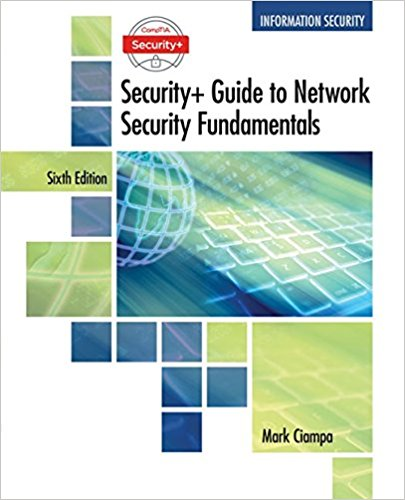
\includegraphics[width=1in]{img/cis249}} & \hangindent .4in \textbf{Textbook:} Ciampa, M. (2017). CompTIA Security+ Guide to Network Security Fundamentals (6th edition). Cengage Learning. ISBN-10: 1337288780 $\bullet$ ISBN-13: 978-1337288781.
}